\let\negmedspace\undefined
\let\negthickspace\undefined
\documentclass[journal]{IEEEtran}
\usepackage[a5paper, margin=10mm, onecolumn]{geometry}
%\usepackage{lmodern} % Ensure lmodern is loaded for pdflatex
\usepackage{tfrupee} % Include tfrupee package

\setlength{\headheight}{1cm} % Set the height of the header box
\setlength{\headsep}{0mm}     % Set the distance between the header box and the top of the text

\usepackage{gvv-book}
\usepackage{gvv}
\usepackage{cite}
\usepackage{amsmath,amssymb,amsfonts,amsthm}
\usepackage{algorithmic}
\usepackage{graphicx}
\usepackage{textcomp}
\usepackage{xcolor}
\usepackage{txfonts}
\usepackage{listings}
\usepackage{enumitem}
\usepackage{mathtools}
\usepackage{gensymb}
\usepackage{comment}
\usepackage[breaklinks=true]{hyperref}
\usepackage{tkz-euclide} 
\usepackage{listings}
% \usepackage{gvv}                                        
\def\inputGnumericTable{}                                 
\usepackage[latin1]{inputenc}                                
\usepackage{color}                                            
\usepackage{array}                                            
\usepackage{longtable}                                       
\usepackage{calc}                                             
\usepackage{multirow}                                         
\usepackage{hhline}                                           
\usepackage{ifthen}                                           
\usepackage{lscape}
\begin{document}

\bibliographystyle{IEEEtran}
\vspace{3cm}

\title{1-1.9-8}
\author{EE24BTECH11010 - BALAJI B
}
% \maketitle
% \newpage
% \bigskip
{\let\newpage\relax\maketitle}

\renewcommand{\thefigure}{\theenumi}
\renewcommand{\thetable}{\theenumi}
\setlength{\intextsep}{10pt} % Space between text and floats


\numberwithin{equation}{enumi}
\numberwithin{figure}{enumi}
\renewcommand{\thetable}{\theenumi}

\textbf{Question :} \\ 
The distance between the points \myvec{0 \\ 0} and \myvec{a - b \\ a + b} is   \\

\textbf{Answer :} \\

\begin{table}[h!]    
  \centering
  \begin{tabular}[12pt]{ |c| c| c|c|c|c|}
    \hline
    $X$ & 1 & 2 & 3 & 4 & 5 \\
    \hline
    $P(X)$ & $K$ & 2$K$ & 2$K$ & 3$K$ & $K$ \\
    \hline 
    \end{tabular} 

  \caption{Variables Used}
  \label{tab1.9.19.1}
\end{table}
\begin{align}
    \therefore\vec{P} - \vec{Q} &= \myvec{0 \\ 0 } - \myvec{a - b \\ a + b} = \myvec{b - a \\ -a -b} \\
    \brak{\vec{P - Q}}^\top \brak{\vec{P - Q}} &= \myvec{b-a & -a-b}\myvec{b-a \\ -a-b} \\
    \brak{\vec{P - Q}}^\top \brak{\vec{P - Q}} &= (b - a)^2 + (a + b)^2
\end{align} 
Thus the desired distance is 
\begin{align}
    d = \norm{P - Q} = \sqrt{(b - a)^2 + (a + b)^2}
\end{align}
Assuming the points a = 2 and b = 3 
\begin{align}
    \vec{P} &= \myvec{0 \\ 0} \text{ and }\vec{Q} = \myvec{-1 \\ 5} \\
    d &= \norm{P - Q} = \sqrt{(3 - 2)^2 + (2 + 3)^2}\\
    d &= \sqrt{26}
\end{align}

\begin{figure}[h!]
   \centering
   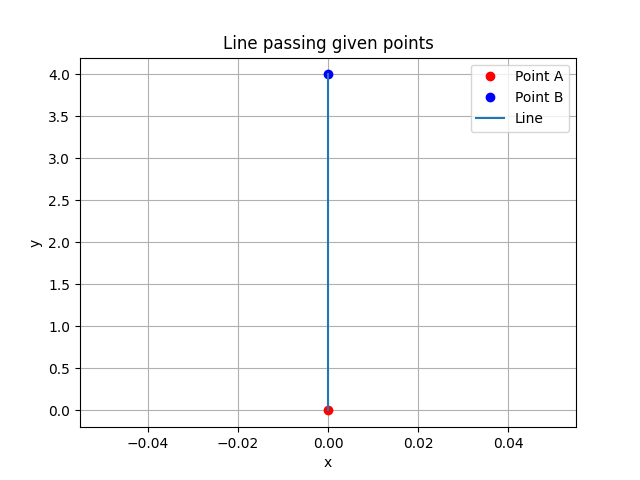
\includegraphics[width=0.7\linewidth]{figs/fig.png}
   \caption{Plot of the line passing through  P and Q}
   \label{stemplot}
\end{figure}

\end{document}

